\documentclass[a4paper, 12pt]{report}

\usepackage{amsfonts} % if you want blackboard bold symbols e.g. for real numbers
\usepackage{graphicx} % if you want to include jpeg or pdf pictures
\usepackage{lmodern}
\usepackage{amsmath}
\usepackage{amssymb}
\usepackage{algorithmic}
\usepackage{algorithm}
 %%% Time-stamp: <mainrep.tex 13:08, 25 May 2009 by P. Sunthar>

%%% $Log:$




%%% Some commonly used packages (make sure your LaTeX installation
%%% contains these packages, if not ask your senior to help installing
%%% the packages)

\usepackage[bookmarks,%
            a4paper,%
            breaklinks,%
            backref=false,%
            dvips,ps2pdf,%
            pdfhighlight=/I,%
            pdffitwindow=true,%
            pdfstartview=Fit,%
            pdfcenterwindow=true,%
            linkbordercolor={1 0 1},%
            %colorlinks,%
            pdftitle=Progress report%
            pdfauthor=Kim Svensson]%
            {hyperref}



\usepackage{amsmath}
\usepackage{epstopdf}
\usepackage{natbib}
\usepackage{booktabs}
\usepackage{graphicx}
\graphicspath{{expt/}}
\usepackage{setspace}
\usepackage{natbib}
\usepackage{times}
\usepackage[varg]{txfonts}
\usepackage[utf8]{inputenc}

%%% Macro definitions for Commonly used symbols
\newcommand{\etas}{\ensuremath{\eta_{\mathrm{s}}}}
\newcommand{\tdegree}{A project progress report submitted for the award of\\}
\newcommand{\degree}{\tdegree MEng Computer Science\\*}
\newcommand{\texam}{Second examiner: }
\newcommand{\exam}{\texam Dr Srinandan Dasmahapatra}
\newcommand{\tsupervisor}{Project supervisor: }
\newcommand{\supervisor}{\tsupervisor Dr.\ Sarvapali D. Ramchurn}
\newcommand{\school}{Electronics and Computer Science \\*
Faculty of Physical and Applied Sciences\\*
University of Southampton\\*}


\newenvironment{changemargin}[2]{%
\begin{list}{}{%
\setlength{\topsep}{0pt}%
\setlength{\leftmargin}{#1}%
\setlength{\rightmargin}{#2}%
\setlength{\listparindent}{\parindent}%
\setlength{\itemindent}{\parindent}%
\setlength{\parsep}{\parskip}%
}%
\item[]}{\end{list}}


\begin{document}

\author{Kim Svensson}
\date{\today}
\title{Combinatorial optimization of NP-hard problems using dynamic GPU programming}

\makeatletter
\begin{titlepage}
\begin{changemargin}{-2cm}{-2cm}
\begin{center}
\LARGE\school %

\LARGE
\vfill
\@author \\*
\@date \\*
\doublespacing
\@title \\*
\vfill
\singlespacing
\supervisor \\*
\exam \\*
\vfill
\degree
\end{center} 
\end{changemargin}
\end{titlepage}
\makeatother

\pagenumbering{arabic}
\begin{abstract}
Solving problems that have an exponential growth in time and space have always been a difficulty as the advancement in computing speed only allows for a small increase of the problem size. The advent of parallel computing using a GPU have enabled a speedup when it comes to problems which have some data and computation independent parts.
The purpose of this project is to develop and evaluate dynamic programming algorithms suitable for parallel computation to find an optimal solution in the domain of complete coalition formation and combinatorial auctions. The heterogeneous algorithm is run using the Nvidia CUDA framework and preliminary result shows a substantial difference and is publishable results.

\end{abstract}
\tableofcontents
\newpage
\section{Introduction}

With NP-hard problems and algorithms with a complexity class of P or greater, a doubling in CPU speed allows only for a small change in sample size due to the nature of such problems, as execution speed and sample size of an algorithm is mutually exclusive.
As such, computer scientists have to find other ways of computing difficult problems on large sets of data.
The traditional approach has been to increase the CPU speed and the number of CPUs.
However, such implementation is often costly and suffers from latency and architectural difficulties.
As the GPU function like a single instruction multiple data (SIMD) architecture with up to thousands of programmable cores, researchers have used GPUs to run concurrent algorithms faster than the equivalent sequential algorithms designed for CPUs. Especially since the development of NVIDIA CUDA and OpenCL implementation in both hardware and software.
This advance in computer science can allow for large computations that were previously unfeasible by leveraging the parallel nature of GPUs. In combinatorial optimization the problem consist of finding the optimal solution for a problem, which for a large set of data can be unfeasable if the problem is NP-hard.
\section{Background}
\subsection{Combinatorial Auctions}
Sometimes auctioneers may sell out several of their assets at the same time such as the government selling parts of the radio spectrum. The bidder may then make offers on subsets of the assets. The problem occurs when there is a large amount of assets being sold while the amount of bids are non-trivial. As for each bid, it have to made sure that no other bid that only accuires a subset of the original bid is greater.
The goal is therefore to calculate which set of pairwise disjoint bids gives the most revenue to the auctioneer.\\*
\newpage
 Consider that the auctioneer is selling the assets $\clubsuit , \diamondsuit$ and $\heartsuit$. The bids collected are as following:

\begin{table}[htb]
\centering
\begin{tabular}{ l | c}
\hline  
Set & Bid \\
\hline
$\clubsuit$ & 3 \\
$\diamondsuit$ & 2 \\
$\heartsuit$ & 6 \\
$\clubsuit, \diamondsuit$ & 7 \\
$\clubsuit, \heartsuit$ & 7 \\
$\diamondsuit, \heartsuit$ & 4 \\
$\clubsuit, \diamondsuit, \heartsuit$ & 6 \\
\end{tabular}
\caption{This table shows some data}
\label{tab:bids}
\end{table}
The winning bid configuration would be the following set:$ \{\{\heartsuit\},\{\clubsuit , \diamondsuit\}\}$ with a total sum of $7 \{\clubsuit , \diamondsuit\}+6 \{\heartsuit\} = 13$ as it is the maximum sum of all combinations of disjoint sets. Where all complete disjoints sets are:

\begin{table}[htb]
\centering
\begin{tabular}{c | l }
\hline
Complete disjoint set & Sum\\
\hline
$\{\{\heartsuit \},\{\clubsuit , \diamondsuit \}\} $ & 13 \\
$\{\{\diamondsuit \},\{\clubsuit , \heartsuit \}\} $ & 9 \\
$\{\{\clubsuit \},\{\diamondsuit , \heartsuit \}\} $ & 7 \\

$\{\{\clubsuit,\diamondsuit , \heartsuit \}\} $ & 6 \\
$\{\{\clubsuit \},\{\diamondsuit \}, \{ \heartsuit \}\} $ &  11
\end{tabular}
\caption{This table shows some data}
\label{tab:disjoint}
\end{table}

The way you calculate the optimal solution for combinatorial auctions is by given any set, find the greates sum for the whole collection of pairwise disjoint subsets of that set and evaluate if it is greater than the set itself. This procedure is done for all sets to finally find a final solution that is the optimal one which give the largest revenue to the auctioneer.
\subsection{Complete Coalition Formation}
Coalition structure generation is a complete analogy to combinatorial auction but from another perspective. It can be translated in such that the assets become agents, an agent can be described as a entity that act on its own, be it a person or a node in a network. A set of assets subjected to a bid is called a coalition formation, in short when two or more agents form a coalition to be regarded as one entity. The auction bid will be translated to coalition value, which means the value gained when two ore more agents form a coalition. Analogous to the previous example, given N agents, generate a set of coalition formations such that the outcome is optimal in regards to the coalition formation value. This however will be an extreme challenge as the number of possible partitions grows exponential with $n$, specifically $O(n^n)$~\cite{rahwan2008improved}. One algorithm to solve this problem in $O(n^3)$ time is called the Dynamic Programming(DP) algorithm~\citep{rothkopf1998computationally} described in algorithm ~\ref{DP}.

It works with the dynamic programming bottom-up approach where you start at sets with cardinality 2 and see if the sum of the pair-wise disjoint subsets value is greater than the original set. If it is assign the new sum to that set. With this principle, all sets with the greatest sum will be carried forward when the cardinality of the sets increases. This algorithm is deterministic, meaning that even if there is only one bid, the computation will take the same time as 1000 bids for a given set of agents. \\

\begin{algorithm}
\caption{Dynamic Programming algorithm \label{DP}}
INPUT: $b(C)$ the bids for all sets $C \subseteq A$ where $A$ is the set of assets.\\*
VARIABLES: $f$ a function that maps from a subset $C \subseteq A$ to a value\\*
$O$ a function that maps from a subset $C \subseteq A$ to the subset that maximize the value for set $C$.
\begin{algorithmic}[1]
\STATE\algorithmicfor\ all $x \in A$, \algorithmicdo $f(\{x\}):= b(\{x\}),O\{x\}:= \{x\}$ \algorithmicendfor
\FOR{$i := 2$ to $n$}
\FOR{all $C \subseteq A: \vert C \vert == i$}
\STATE $f(C) := max\{f(C\backslash C')+f(C'):C'\subseteq C \wedge 1 \leq \vert C' \vert \leq \dfrac{\vert C \vert}{2}\}$ \label{lst:line:a}
\STATE\algorithmicif $f(C) \geq b(C)$ \algorithmicthen\ $O(C) := C^{*}$ \hfill Where $C^{*}$ maximizes right hand side of line~\ref{lst:line:a} \algorithmicendif
\STATE\algorithmicif $f(C) < b(C)$ \algorithmicthen\ $f(C) := b(C)\wedge O(C) := C$ \algorithmicendif
\ENDFOR
\ENDFOR
\end{algorithmic}
\end{algorithm}

\subsection{NVIDIA CUDA}
CUDA (formerly known as Compute Unified Device Architecture) is a framework by NVIDIA equivalent to OpenCL which allows for C,C++ and FORTRAN code to be compiled and run on its Graphics Processing Units (GPUs). As GPUs are many-core processors designed to handle large amount of independent data when running a graphics program, it is advantageous to utilize such architecture to handle general purpose algorithms to solve complex problems with parallel nature. This architecture is described as Single Instruction Multiple Threads (SIMT) which could be seen similar to the Single instruction, multiple data (SIMD) architecture. The fundamental difference is that with SIMT, branch divergence is allowed.

The CUDA architecture consist of a scaled array of Streaming Multiprocessors (SM), where each SM contains from 8 cores to 192 programmable cores depending on the GPU version. Where one GPU can have several SMs. When launching a kernel which can be seen as a function call, the threads assigned are divided up into blocks of threads. Each block gets assigned to an SM to be processed resulting in two blocks from the same kernel can be running concurrently on two different SMs. If there is no SM freely available the block will be put into a queue. The next thing to note is that each block is divided into warps of 32 threads which is scheduled by the warp scheduler. The reason is to hide memory read and write latency as while one warp is blocked waiting for data, another warp can run its instructions. Therefore the size of each threadblock should be a multiple of 32 threads to allow full utilisation of the warp.


\section{Literature review}
With Combinatorial auctions and multi-agent coalition formation being combinatorial optimization problem, an literature review was conducted to find relevant publications in the area.

The DP algorithm have been the best algorithm to solve coalition structur generation problem in deterministic time until the advent of the Improved Dynamic Programming(IDP) algorithm by Rahwan, T. and Jennings, N.R.~\cite{rahwan2008improved}. It uses a simple, yet novel way to determine which coalition structures should be examined, reducing the edges traveled in the directed graph, which allows for a shorter runtime yet conserves the optimality of the DP algorithm.  \\*

Solving the incomplete combinatoral auctions using non-determenistic algorithms trade-offs have to be made. Constructing the bids in a tree structure is common, but how the heuristics is formed to traverse and search the tree for the optimal solution is often quite different. One algorithm called CPLEX is using a heuristic A* search algorithm which explores the most promising branch first. 
This however suffers from exponential memory requirement, however if the problem can fit into memory it finds a solution faster on hard problems than the pruposed CABOB algorithm. CABOB uses a depth-first branch-and-bound heuristic which only require the current branch investigated to be held in the memory. This gives the algorithm a linear memory requirement with regards to the depth of the branch. However as this is an depth-first algorithm, the worst case scinario occurs with a large depth of the tree which is not precent in the CPLEX algorithm. However for a larger problem the CABOB algorithm is most suited as CPLEX require a vast amount of memory to function~\cite{sandholm2002algorithm}.\\*

One of the few papers regarding a distributed or concurently run algorithm for coalition structure generation used 14 dualcore workstations~\cite{michalak2010distributed}. Their solution only had a runtime from 11\% to 4\% of the centralised variant. However as the computers comunicated over the ethernet, latancies may vastly affect the runtime, which could be improved by running it concurrently on a GPU.

Using the GPU together with dynamic programming have been used before to solve similar combinatorial optimization problems. Boyer, V et al successfully implemented and solved the knapsack problem with a great reduction in run-time~\cite{boyer2012solving}. They also introduced ways of reducing memory occupancy which enable computation of much larger data sets as well as reducing the bandwidth utilized allowing for a faster processing speed. This is one of the most important aspects of GPU programming as you are first limited to the amount of memmory the GPU have, but also in order to increase the effective bandwidth of the algorithm.





\section{Work}
My work has been written in ANSI C, the reason is large amount of experience in the language but also the fact that one of the native languages supported by the CUDA framework is the C programming language.
To this point I have implemented the algorithm called the Dynamic Programming (DP) algorithm by Rothkopf, M.H et al~\cite{rothkopf1998computationally} which is used to solve combinatorial auctions, but it can also be used for complete coalition formation as described before. It was first implemented as a sequential algorithm to allow for a baseline to compare execution speed by. But also to gain knowledge about the algorithm to allow easier transition towards a parallel version. The algorithm I have derived that run on the GPU is represented by the max function at line~\ref{lst:line:a} of the DP algorithm, which consists of generating pairwise disjoint subsets from a given set, and then calculated the value the disjoint sets give and compare it to the original set. 

\thispagestyle{empty}

\thispagestyle{empty}
\pagestyle{empty}
%\begin{algorithm}
%\caption{Calculate the }asd
\subsection{Algorithm}
\textbf{Input}

$f$\hfill The array which holds the bids

$O$\hfill The step array that holds set configurations

$ \Phi $ \hfill A reference to an maximum value bucket unique for each kernel

$C$\hfill The set to do subset construction on

$\Psi$\hfill The maximum subset construction index


\textbf{Variables} 

$\lambda$ \hfill How many bids should be evaluated per thread

$\Upsilon$ \hfill A shared array containing threads maximum bid values

$\Delta$ \hfill A shared array containing threads maximum bid subsets

$\upsilon$ \hfill A local array containing one of the threads bid value

$C'$ \hfill A local array containing one of the threads bid subsets

$bid = blockIdx.x$ \hfill Which block the threads belong to

$bdim = blockdim.x$ \hfill How many threads inside the block

$tid = threadIdx.x$ \hfill The thread index inside the block

$\psi := \lambda*(tid+bdim*bid)$ \hfill Initial subset construction index

\textbf{Start of algorithm}
\begin{algorithmic}[1]
\STATE $\Delta _{tid} := \Upsilon _{tid} := 0$ \hfill Initialize values to zero
\IF{$\psi \leq \Psi$} 
\FOR {$i := 1$ to $\lambda$}
\STATE $C'_{i} := (\neg C+\psi) \bigcap C$ \label{lst:line:subset} \hfill Integer subset construction
\IF{$ \vert C'_{i} \vert \leq \dfrac{\vert C\vert }{2} \wedge \psi \leq \Psi$}
\STATE $\upsilon _{i} := f[C/C'_{i}]+f[C'_{i}]$ \hfill Set the split subset coalition value
\ENDIF 

\IF {$\upsilon _{i} > \Upsilon _{tid}$} 
\STATE $\Upsilon _{tid} := \upsilon _{i}$  \hfill Set value if $\upsilon _{tid}$ is greatest so far
\STATE $\Delta _{tid} := C'_{i}$ \hfill Set subset if $\upsilon _{tid}$ is greatest so far
\ENDIF
\STATE $\psi := \psi + 1$ \hfill Increment by one
\ENDFOR
\ENDIF

\STATE $syncthreads$ \hfill make sure all threads have finished
\FOR {$i := bdim >> 1$ to $0$} \label{lst:line:mid}
\IF{$tid < i$} \label{lst:line:midmid}
\IF{$\Upsilon _{tid} \leq \Upsilon _{tid+i}$} \label{lst:line:midmidmid}
\STATE $\Delta _{tid} := \Delta _{tid+i}$ 
\STATE $\Upsilon _{tid} := \Upsilon _{tid+i}$
\ENDIF
\ENDIF
\STATE $syncthreads$ \hfill make sure all threads have finished
\STATE $i := i >> 1$ \hfill bit-shift i once to the right \label{lst:line:midlast}
\ENDFOR \label{lst:line:midend}
\IF{$tid == 0$} \label{lst:line:last}
\STATE\algorithmicif{$\Upsilon _0 == 0$} \algorithmicthen\ {$ exit$}
\algorithmicend\ \algorithmicif \hfill exit if the bid is zero
\STATE\algorithmicif{$f_C > \Upsilon _0$} \algorithmicthen\ {$ exit$} 
\algorithmicend\ \algorithmicif \hfill exit if the bid is less than for C
\IF{$atomicMax(\Phi,\Upsilon _0) < \Upsilon _0$}  \label{lst:line:lastmid}
\STATE $O_C = \Delta _0$ \hfill Sets the current optimal step in global memory
\STATE $f_C = \Upsilon _0$ \hfill Sets the current optimal value in global memory
\STATE $threadfence$ \hfill make sure all threads see the changes
\ENDIF 

\ENDIF \label{lst:line:lastend}
\RETURN $O,f$
\end{algorithmic}
%\end{algorithm}
Line~\ref{lst:line:subset} represent how the subset construction is made, it starts by taking the inverse of the integer $C$, add together the subset construction index $\psi$, and finally apply a bit-wise AND with $C$ to get a guaranteed subset of $C$. This implementation suffers though from generating subsets of greater cardinality needed, but testing have shown that the instruction overhead for generating these unwanted subsets only account for 18\% to 8\% overhead as shown by figure~\ref{overhead}. The reason for representing a set as an integer was inspired by [knappsack] due to the substantial lower memmory reqired to store a set as an integer rather than an array of integers.\\*
The code from~\ref{lst:line:mid} to~\ref{lst:line:midend} details how to do a reduction among all threads inside a block to find the maximum value from all of the subset constructions the threads have previously done. Where for each cycle of the loop, half of the threads will compare its value to a corresponding inactive thread and set its value and subset to whichever value is largest. Then it will reduce the number of active threads by half and continues until there is no more threads to be active. The loop will run $log(n)$ times where $n$ is the number of threads in the block.\\* Lines~\ref{lst:line:last} to~\ref{lst:line:lastend} represent how each block of a kernel update their maximum value and subset to the global memory for all the consecutive kernels to see. Beginning at line~\ref{lst:line:last}, here only the thread with an id of zero will pass in order to reduce the memory bandwidth but also as there is only need for one thread to update the global memory. Line~\ref{lst:line:lastmid} ensures that only a bigger value can be set by first querying the bucket for this kernel, if it is bigger it can continue to set the global memory. The reason for the atomic function is due to that blocks from the same kernel can and will run concurrently, therefore it will cause race conditions.

This algorithm have been derived through several iterations to find the right balance between amount of registers used, the number of times memory is accesed and how many coalitions should each thread evaluate. 
\section{Result}
\subsection{Experimental Setup}
The evaluation of the CUDA DP algorithm is conducted on a NVIDIA GTX 660TI GPU with 7 streaming processors for a total of 1344 cores and memory capacity of 2GB, the maximum blocksize is set to 256 threads to allow maximum occupancy on the GPU. The CPU DP algorithm is run single threaded on a INTEL XEON W3520 with a clockspeed of 2.67GHz with 32KB L1, 256KB L2 cache. The way the data is structured and stored is identical between both implementations and the time is measured more than once. The early test result show an graph of the logarithmic runtime in base 10 for an increasing number of agents.


\subsection{Evaluation}

\begin{figure}[htb]
\centering
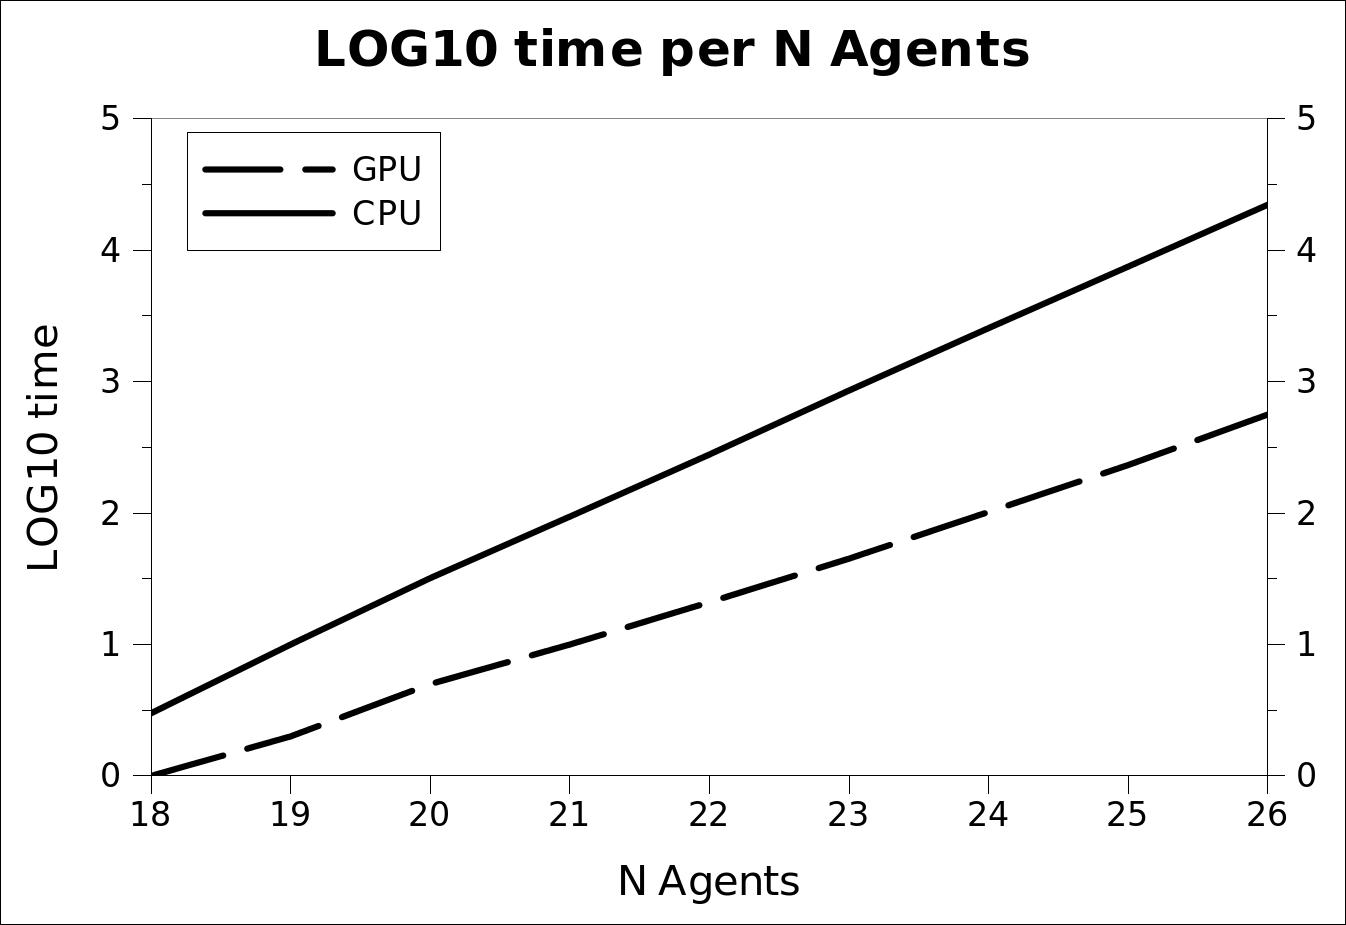
\includegraphics[width=0.7\linewidth]{loggraph.jpg}
\caption{LOG10 run-time per N Agents\label{log}}
\end{figure}


As it stands now, the algorithm that is running using the CUDA framework have an substantial performance increase as shown in figure~\ref{log}. As seen from the figure, the slope of the CPU and GPU lines diverge, indicating an different growth rate for an increase of n, thus having a different time complexity. Empirical measurement show that for each increase in n, the run-time for the CPU increase by three. While the GPU bound algorithm starts its growth at 2 and the growth increases to 2.42 at 25 agents. \\*
\begin{figure}[htp]
\centering
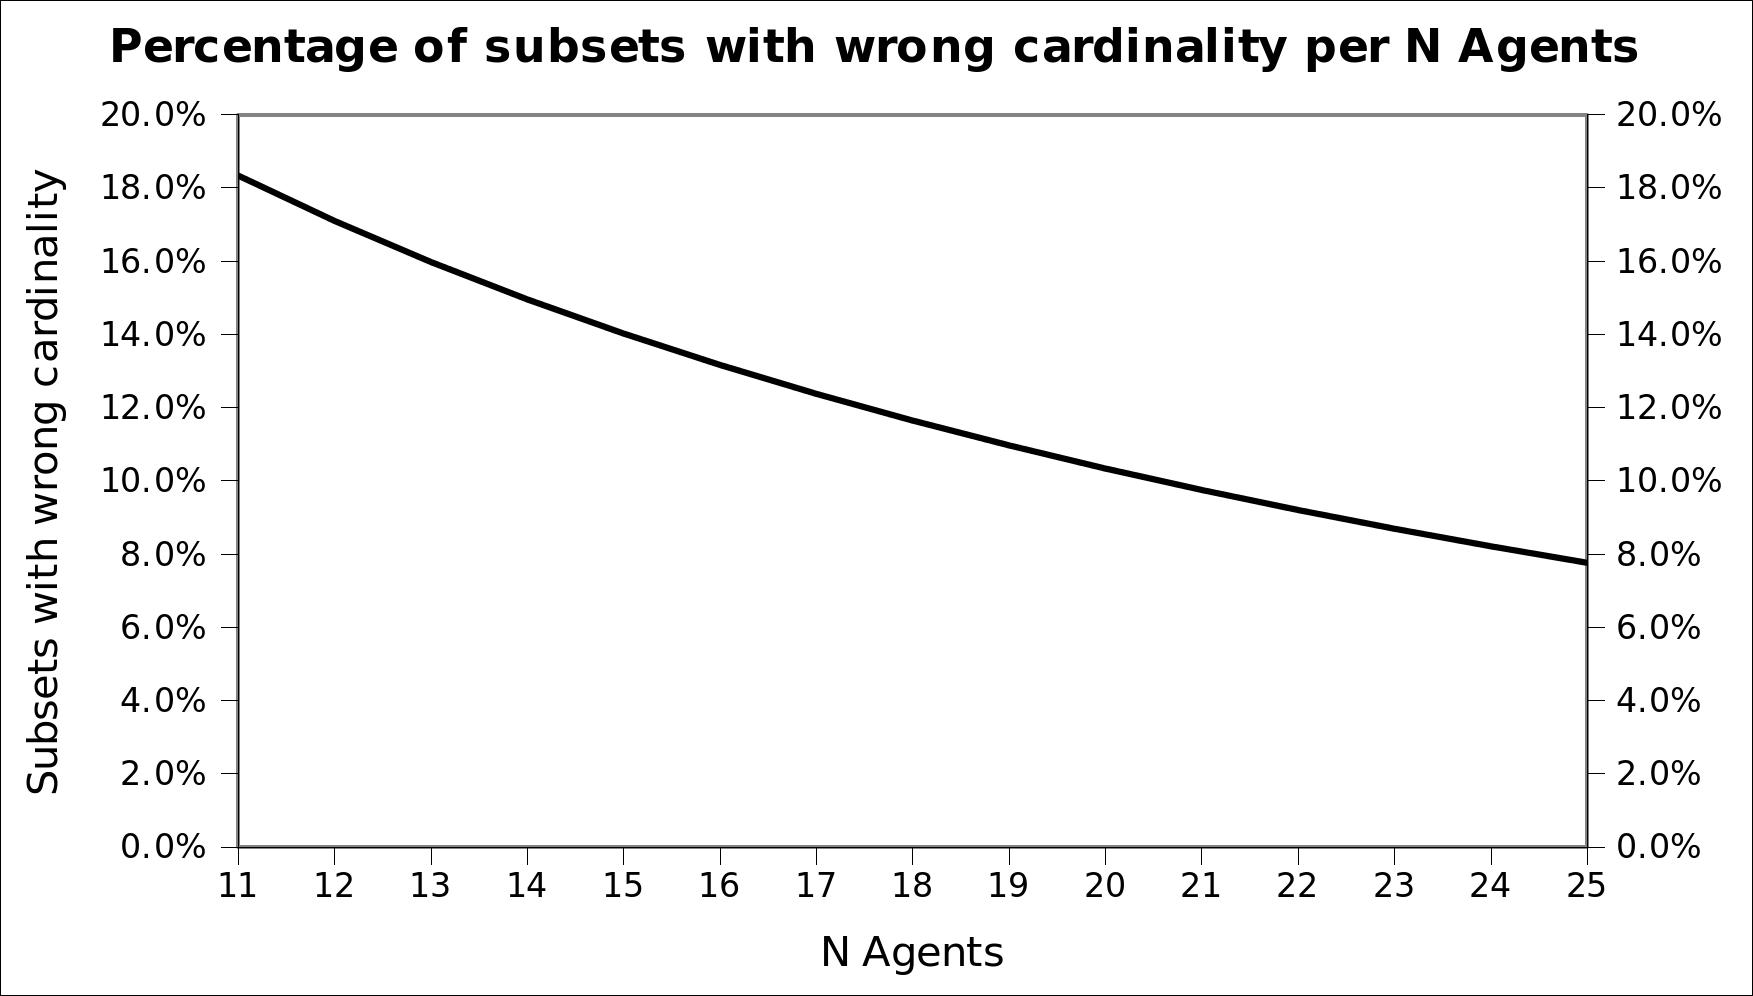
\includegraphics[width=0.7\linewidth]{subset.jpg}
\caption{Percentage of generated subset of wrong cardinality\label{overhead}}
\end{figure}
\linebreak
Figure~\ref{overhead} is the evaluation of line~\ref{lst:line:subset} on how many subsets generated that invalidates the condition $\vert C'_{i} \vert \leq \dfrac{\vert C\vert }{2}$ where $C'_i \subset C$. This is a measure that describe the instruction overhead for that particular part of the algorithm, and as it stands now with the algorithm being limited by memory latency due to random access, this instruction overhead can be considered negligible. This measure however does not take into account any duplicate subsets that are occasionally generated.
\section{Future work}
As the closest algorithm that is regarded faster than the DP algorithm is the IDP algorithm \citep{rahwan2008improved} that have shown a promising reduction in evaluated coalitions. The next step would be to translate my current work to an algorithm that utilizes the IDP technique. This will be both done for the CPU and GPU implementation and later on compared and evaluated to the DP algorithm. However as it is fairly similar to the DP algorithm, implementation should be trivial and further goals need to be determined.\\ As the current work only works for a small number of agents but the complete set of coalitions, the next step would be to implement an algorithm to solve realistic combinatorial auctions with an relative large number of agents and low number of coalition structures. As the Cabob algorithm uses a branch by branch evaluation heuristic that are independant of each other. Such algorithm would be more than suitable to be implemented to run concurrently. \\
Due to the promising results gained, a further more robust testing facility will be programmed to ensure the absolute correctness of my algorithm. If the results stays promising a paper will be written to try and publish the results.


\bibliographystyle{plain}
\bibliography{ref}

\newpage
\begin{figure}[htp]
\centering
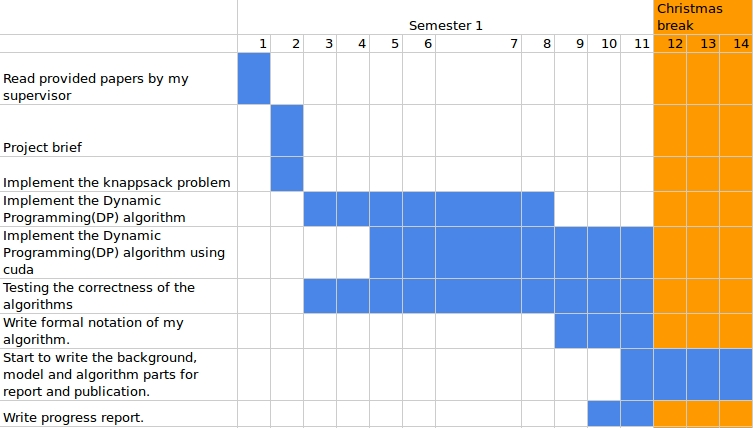
\includegraphics[width=\linewidth]{sem1.jpg}
\caption{Semester 1}
\end{figure}
\begin{figure}[htp]
\centering
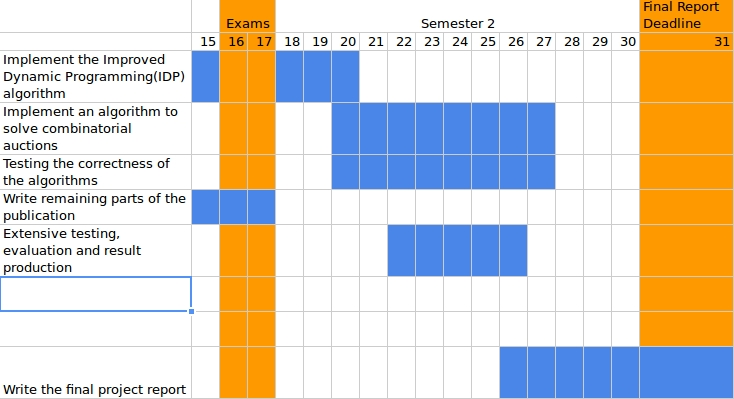
\includegraphics[width=\linewidth]{sem2.jpg}
\caption{Semester 2}
\end{figure}
\begin{figure}[htp]
\centering
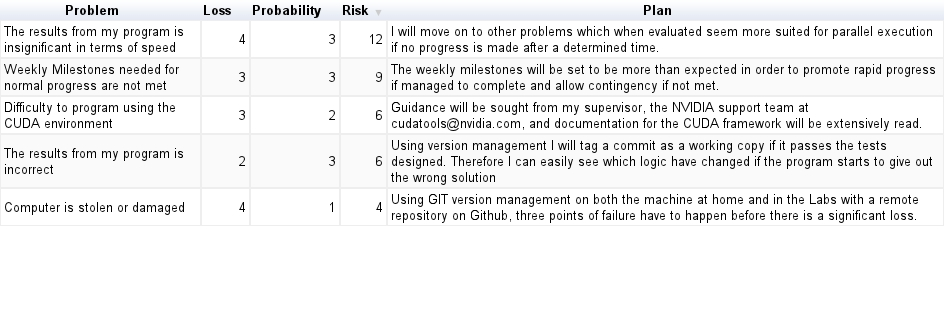
\includegraphics[width=\linewidth]{risk.jpg}
\caption{Risk assessment}
\end{figure}

\end{document}
